\documentclass[tikz]{standalone}

\usepackage{amsmath}
\usepackage{unicode-math}
\usepackage{mathtools}
\usepackage{derivative}

\setmainfont{Stix Two Text}
\setmathfont{Stix Two Math}

\usetikzlibrary{arrows.meta,fit,positioning}

\renewcommand{\familydefault}{\sfdefault}

% prefix equation numbers with section number
\numberwithin{equation}{section}

\DeclarePairedDelimiter{\ceil}{\lceil}{\rceil}
\DeclarePairedDelimiter{\floor}{\lfloor}{\rfloor}
\DeclarePairedDelimiter{\abs}{\lvert}{\rvert}
\DeclarePairedDelimiter{\norm}{\lVert}{\rVert}
\DeclarePairedDelimiter{\bra}{\langle}{\rvert}
\DeclarePairedDelimiter{\ket}{\lvert}{\rangle}
\DeclarePairedDelimiter{\expval}{\langle}{\rangle}
\DeclarePairedDelimiter{\norder}{\mathcolon}{\mathcolon}
\DeclarePairedDelimiter{\anorder}{\typecolon}{\typecolon}
	
\newcommand{\laplace}{\mbfnabla^2}
\newcommand{\trans}{{\scriptscriptstyle\mathsf{T}}}

\newcommand{\vdot}{\cdot}
\newcommand{\vcross}{\vectimes}
\newcommand{\vb}[1]{\symbfup{#1}}
\newcommand{\vu}[1]{\hat{\vb{#1}}}
\newcommand*\dd[2][\relax]{\mathop{\ifx\relax#1\odif{#2}\else \odif[order={#1}]{#2}\fi\,}}

\newcommand{\vacuum}{\ket*{\vb{0}}}

\DeclareMathOperator{\trace}{Tr}
\DeclareMathOperator{\sinc}{sinc}

\AtBeginDocument{
	\let\Re\relax
	\let\Im\relax
	\DeclareMathOperator{\Re}{Re}
	\DeclareMathOperator{\Im}{Im}

	\renewcommand{\div}{\mathop{\mbfnabla\vdot}}
	\newcommand{\curl}{\mathop{\mbfnabla\vectimes}}
}

\DeclarePairedDelimiterX{\comm}[2]{[}{]}{#1,#2}

\DeclarePairedDelimiterX{\braket}[2]{\langle}{\rangle}{#1\delimsize\vert#2}
\DeclarePairedDelimiterX{\ketbra}[1]{\lvert}{\rvert}{#1\rangle\delimsize\langle#1}



\begin{document}
	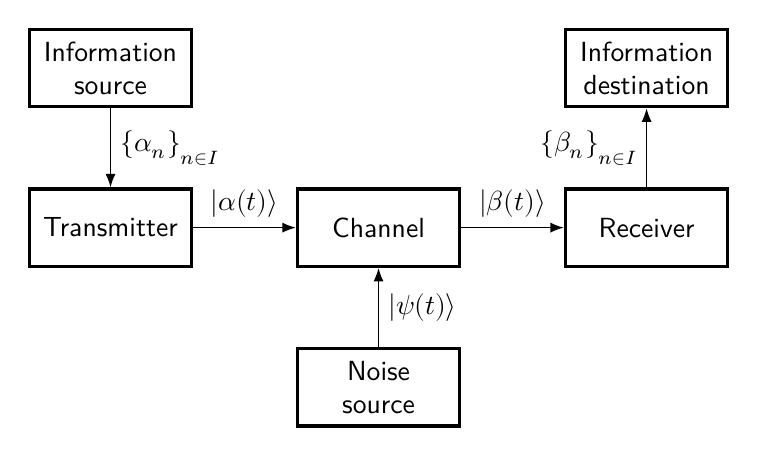
\begin{tikzpicture}[
		node distance=1cm,
        block/.style={draw, very thick, fill=white, minimum height=28pt, minimum width=58pt, text width=52pt, align=center},
        arrow/.style={-Latex},
	]
		\node[block] (src) {Information source};
		\node[block, below=of src] (tx) {Transmitter};
		\node[block, right=1.3cm of tx] (ch) {Channel};
		\node[block, right=1.3cm of ch] (rx) {Receiver};
		\node[block, above=of rx] (dst) {Information destination};
		\node[block, below=of ch] (ns) {Noise source};
		
		\draw[arrow] (src) -- (tx) node[midway, right] {$\left\{\alpha_n\right\}_{n\in I}$};
		\draw[arrow] (tx) -- (ch) node[midway, above] {$\ket{\alpha(t)}$};
		\draw[arrow] (ch) -- (rx) node[midway, above] {$\ket{\beta(t)}$};
		\draw[arrow] (rx) -- (dst) node[midway, left] {$\left\{\beta_n\right\}_{n\in I}$};
		\draw[arrow] (ns) -- (ch) node[midway, right] {$\ket{\psi(t)}$};;
	\end{tikzpicture}
\end{document}
